\documentclass[tikz,border=5pt]{standalone}
\usepackage[T1]{fontenc}
\usepackage{lmodern,amsmath,amssymb}
\usetikzlibrary{arrows.meta,calc,positioning,fit,backgrounds,shapes.geometric,matrix,decorations.pathreplacing,patterns}
\definecolor{ink}{gray}{0.08}
\definecolor{wash}{gray}{0.965}
\definecolor{soft}{gray}{0.45}
\tikzset{box/.style={draw=ink,line width=.65pt,fill=white,align=center,inner sep=4pt,outer sep=0pt,font=\small},flow/.style={draw=ink,line width=.65pt,-{Latex[length=1.8mm,width=1.3mm]},rounded corners=2pt},annotation/.style={font=\scriptsize,text=soft,align=center},groupbox/.style={draw=soft,dashed,line width=.45pt,fill=wash}}
\begin{document}
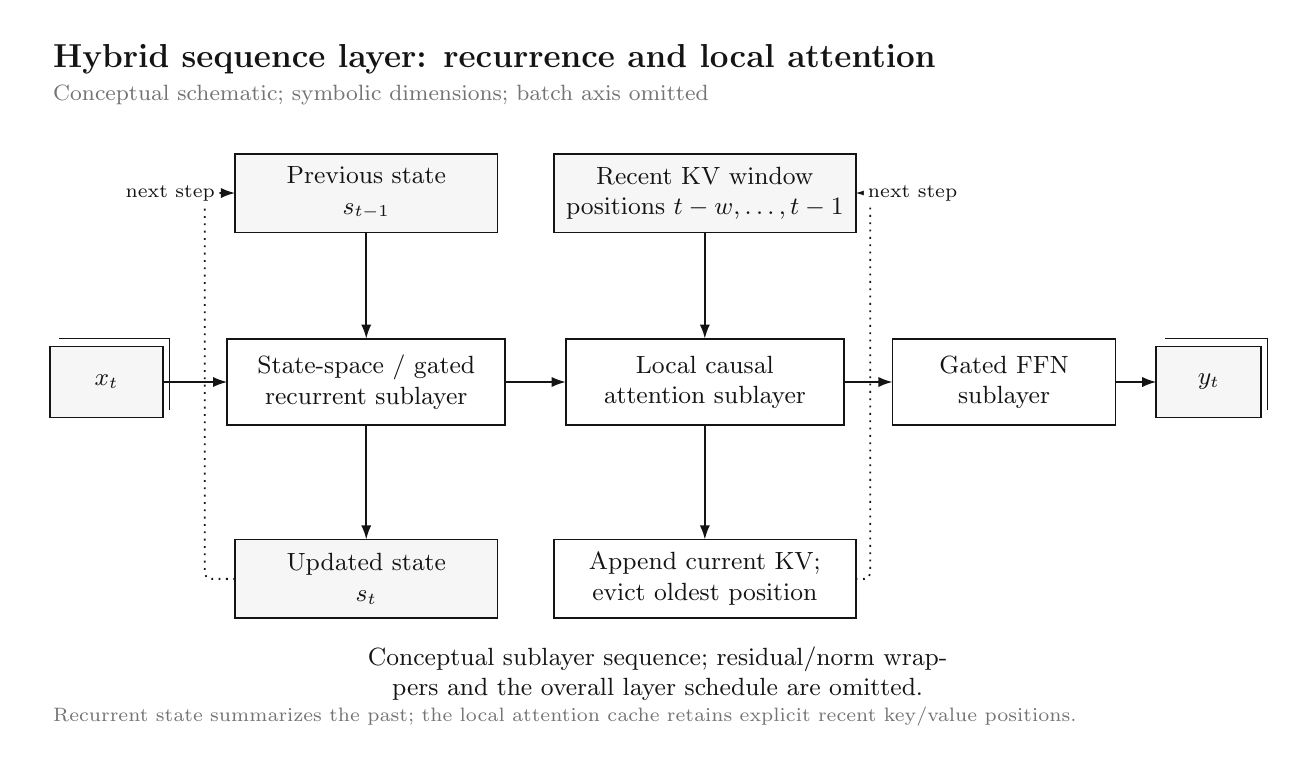
\begin{tikzpicture}[x=1cm,y=-1cm,font=\rmfamily,text=ink]

\path[use as bounding box] (0,0) rectangle (16,9);
\node[anchor=west,font=\large\bfseries] at (.2,.4) {Hybrid sequence layer: recurrence and local attention};
\node[anchor=west,font=\footnotesize,text=soft] at (.2,.85) {Conceptual schematic; symbolic dimensions; batch axis omitted};
\begin{pgfonlayer}{background}
\end{pgfonlayer}
\node[box,fill=wash,minimum width=1.4cm,minimum height=0.9cm,text width=1.15cm] (x) at (1.0,4.5) {$x_t$};
\draw[ink,line width=.4pt] (0.4,3.9499999999999997) -- (1.8,3.9499999999999997) -- (1.8,4.8500000000000005);
\node[box,minimum width=3.5cm,minimum height=1.1cm,text width=3.25cm] (rec) at (4.3,4.5) {State-space / gated\\recurrent sublayer};
\node[box,minimum width=3.5cm,minimum height=1.1cm,text width=3.25cm] (attn) at (8.6,4.5) {Local causal\\attention sublayer};
\node[box,minimum width=2.8cm,minimum height=1.1cm,text width=2.55cm] (ffn) at (12.4,4.5) {Gated FFN\\sublayer};
\node[box,fill=wash,minimum width=1.3cm,minimum height=0.9cm,text width=1.05cm] (y) at (15,4.5) {$y_t$};
\draw[ink,line width=.4pt] (14.45,3.9499999999999997) -- (15.75,3.9499999999999997) -- (15.75,4.8500000000000005);
\node[box,fill=wash,minimum width=3.3cm,minimum height=1.0cm,text width=3.05cm] (prev) at (4.3,2.1) {Previous state\\$s_{t-1}$};
\node[box,fill=wash,minimum width=3.8cm,minimum height=1.0cm,text width=3.55cm] (window) at (8.6,2.1) {Recent KV window\\positions $t-w,\ldots,t-1$};
\node[box,fill=wash,minimum width=3.3cm,minimum height=1.0cm,text width=3.05cm] (next) at (4.3,7.0) {Updated state\\$s_t$};
\node[box,minimum width=3.8cm,minimum height=1.0cm,text width=3.55cm] (newkv) at (8.6,7.0) {Append current KV;\\evict oldest position};
\node[align=center,inner sep=0pt,outer sep=0pt,font=\small,minimum width=14cm,minimum height=0.4cm,text width=13.75cm] (note9) at (8,8.2) {Conceptual sublayer sequence; residual/norm wrappers and the overall layer schedule are omitted.};
\begin{pgfonlayer}{background}
\draw[flow] (x.east) -- (rec.west);
\draw[flow] (rec.east) -- (attn.west);
\draw[flow] (attn.east) -- (ffn.west);
\draw[flow] (ffn.east) -- (y.west);
\draw[flow] (prev.south) -- (rec.north);
\draw[flow] (rec.south) -- (next.north);
\draw[flow] (window.south) -- (attn.north);
\draw[flow] (attn.south) -- (newkv.north);
\draw[flow,dotted] (next.west) -- (2.25,7) -- (2.25,2.1) -- (prev.west) node[midway,left,fill=white,inner sep=1.5pt,font=\scriptsize] {next step};
\draw[flow,dotted] (newkv.east) -- (10.7,7) -- (10.7,2.1) -- (window.east) node[midway,right,fill=white,inner sep=1.5pt,font=\scriptsize] {next step};
\end{pgfonlayer}
\node[anchor=west,align=left,font=\scriptsize,text=soft,text width=15.6cm] at (.2,8.75) {Recurrent state summarizes the past; the local attention cache retains explicit recent key/value positions.};
\end{tikzpicture}
\end{document}
